
\section{Servicios de BaaS y Firebase}
\label{\detokenize{chapter_one/firebase:servicios-de-baas-y-firebase}}\label{\detokenize{chapter_one/firebase::doc}}

\subsection{Backend as a Service}
\label{\detokenize{chapter_one/firebase:backend-as-a-service}}

\begin{remark}
Backend as a service o Mobile Backend as a Service, es un
modelo para proporcionar a los desarrolladores web y
de aplicaciones móviles una forma de vincular estas aplicaciones
al almacenamiento en la nube, servicios analíticos
y/o otras características tales como la gestión de usuarios,
la posibilidad de enviar notificaciones push y la integración
con servicios de redes sociales. Estos servicios son brindados
a través de kits de desarrollo de software (SDK) o
interfaces de programación de aplicaciones (API). 
\end{remark}
Algunos proveedores
de este tipo de cómputo en la nube son Microsoft Azure Mobile Services,
Oracle Cloud (Mobile Service) y \sphinxstylestrong{Firebase}, que es la plataforma
que se usa en este proyecto y por tanto se describe a detalle a
continuación.


\subsection{Firebase}
\label{\detokenize{chapter_one/firebase:firebase}}
Firebase es una plataforma de desarrollo para aplicaciones móviles y web.
Tiene varias tecnologías para mejorar la experiencia de desarrollo de una
aplicación, como la autenticación, base de datos en tiempo real,
almacenamiento en la nube, alojamiento de un sitio estático y funciones en la
nube para ejecutar código de backend.

A pesar de ser una plataforma enfocada principalmente para ser un servicio de
backend para aplicaciones móviles y web, algunos de sus servicios cuentan con
una API REST lo que permite acceder a estos a través de entornos con recursos
restringidos.

De las tecnologías ofrecidas por Firebase, se usan:
\begin{itemize}
\item {} 
Realtime database

\item {} 
Authentication

\item {} 
Hosting

\end{itemize}


\subsubsection{Firebase Realtime Database}
\label{\detokenize{chapter_one/firebase:firebase-realtime-database}}
Firebase Realtime Database es una base de datos alojada en la nube.
Los datos se almacenan en formato JSON y se sincronizan en tiempo real con cada
cliente conectado. Los clientes comparten una instancia de Realtime Database y
reciben actualizaciones automáticamente con los datos más recientes.

Entre las funciones más importantes de este servicio están; la
\sphinxstylestrong{sincronización de datos en tiempo real}, cada vez que los datos cambian,
los dispositivos conectados reciben esa actualización en milisegundos.
Trabajo \sphinxstylestrong{sin conexión}, ya que el SDK hace que los datos persistan en el disco,
y cuando la conexión se restablece, el dispositivo cliente recibe los cambios
faltantes y los sincroniza con el estado actual del servidor.
\sphinxstylestrong{Accesible desde dispositivos cliente}, no se necesita un servidor de
aplicaciones; las opciones de seguridad y validación se definen a través de
reglas de seguridad de Firebase Realtime Database. Y finalmente
el \sphinxstylestrong{escalamiento en varias bases de datos}, que permite dividir la información
en diversas instancias de bases de datos dentro del mismo proyecto de Firebase.

La ruta de implementación de la Realtime Database que está definida en la documentación de Firebase,
es la siguiente:
\begin{enumerate}
\item {} 
Integrar los SDK de Firebase Realtime Database.

\item {} 
Crear referencias de Realtime Database.

\item {} 
Configurar datos y escuchar para detectar cambios.

\item {} 
Habilitar la persistencias sin conexión.

\item {} 
Proteger los datos con las reglas de seguridad de Firebase Realtime Database.

\end{enumerate}


\subsubsection{Firebase Authentication}
\label{\detokenize{chapter_one/firebase:firebase-authentication}}
La mayoría de las aplicaciones necesitan identificar a los usuarios. Conocer la
identidad de un usuario permite que una aplicación guarde sus datos en la nube de
forma segura y proporcione la misma experiencia personalizada en todos los
dispositivos del usuario.

Firebase Authentication proporciona servicios de backend, SDK fáciles de usar y
bibliotecas de IU ya elaboradas para autenticar a los usuarios en tu aplicación.
Admite la autenticación mediante contraseñas, números de teléfono, proveedores
de identidad federados populares, como Google, Facebook y Twitter, y mucho más.

Firebase Authentication se integra estrechamente con otros servicios de Firebase
y aprovecha los estándares de la industria como OAuth 2.0 y OpenID Connect, por
lo que se puede integrar fácilmente con tu backend personalizado.


\paragraph{FirebaseUI Auth}
\label{\detokenize{chapter_one/firebase:firebaseui-auth}}
Puedes permitir que los usuarios accedan a tu aplicación de Firebase con FirebaseUI
como solución de autenticación directa o mediante el SDK de Firebase
Authentication para integrar de forma manual uno o más métodos de acceso en tu
aplicación.

FirebaseUI proporciona una solución de autenticación directa que controla los
flujos de IU para los usuarios que acceden con direcciones de correo electrónico
y contraseñas, números de teléfono y con proveedores de identidad federada
populares, que incluyen el Acceso con Google y el Acceso con Facebook.

El componente de FirebaseUI Auth implementa recomendaciones para la autenticación
en sitios web y dispositivos móviles, lo que puede maximizar la conversión de
acceso y registro de tu aplicación. También maneja casos extremos, como recuperación
y vinculación de cuentas, que pueden tener repercusiones en la seguridad y ser
propensos a generar errores cuando se tratan de manejar correctamente.



\subsubsection{Firebase Hosting}
\label{\detokenize{chapter_one/firebase:firebase-hosting}}
Firebase Hosting proporciona hosting estático, rápido y seguro para tu aplicación web.

Firebase Hosting es un servicio de hosting de contenido web con nivel de
producción orientado a programadores. Con Hosting, puedes implementar aplicaciones web
y contenido estático en una red de distribución de contenido global (CDN) con
un solo comando, en forma rápida y sencilla.

La ruta de implementación para utlizar el servicio de alojamiento 
en una aplicación web es la siguiente:

\begin{enumerate}
\item {} 
Instala Firebase CLI. Con Firebase CLI, es fácil configurar un nuevo proyecto de Hosting, administrar un servidor de desarrollo local y también implementar contenido

\item {} 
Configura un directorio de proyectos. Agrega archivos para tu aplicación web y agrega tus activos estáticos a tu carpeta local de Hosting. A continuación, puedes ejecutar \sphinxcode{firebase serve} para tu sitio en forma local.

\item {} 
Implementa tu sitio. Cuando estés satisfecho con la configuración, ejecuta \sphinxcode{firebase deploy} para subir la última instantánea a nuestros servidores.

\end{enumerate}


\subsubsection{Firebase Console}

La consola de Firebase es una interfaz gráfica de usuario, GUI por sus 
siglas en inglés, para que a través de un navegador se administren
los servicios provistos por Firebase. Esta consola permite a los desarrolladores
crear proyectos, añadir servicios a esos proyectos,
configurarlos, administrar las herramientas, visualizar estadísticas
de las aplicaciones, entre muchas cosas más.

\begin{figure}[ht]
\centering
\caption{Una captura de un proyecto visto desde la consola
de Firebase.}
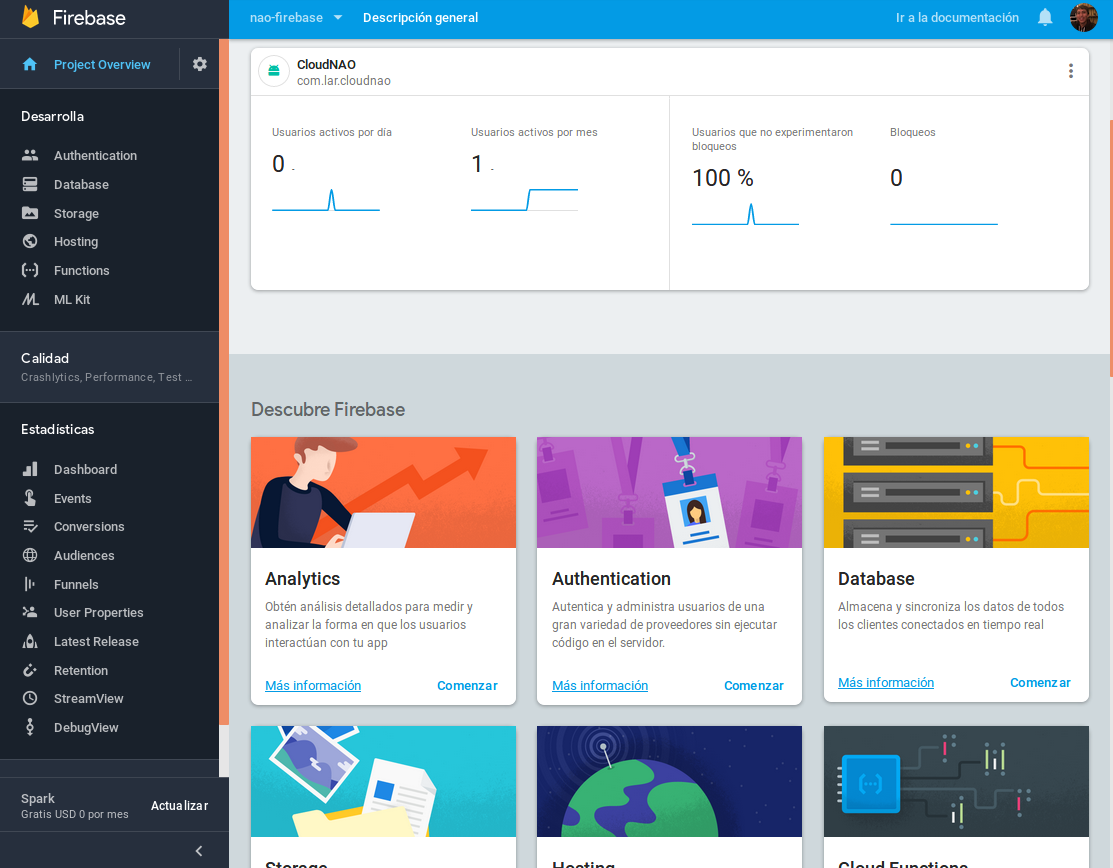
\includegraphics[scale=0.25]{firebase_console}
\end{figure}
